\section{Модель прямоугольного Изинга}

В данном разделе мы будем рассматривать зависимость наблюдаемых модели Изинга от формы решетки: в частности, от отношения сторон в прямоугольной решётке

\subsection{Расчёт критических кумулянтов для модели прямоугольного Изинга}

Кумулянт Биндера для модели Изинга в критической точке расчитывается по формуле:
\begin{equation}
\label{eq:Cumulant}
U_{4} = 1 - \frac{\la m^{4} \ra}{3 * (m^{2})^{2}}
\end{equation}

где $\la m^{2} \ra$ - средний квадрат удельной намагниченности, $\la m^{4} \ra$ - средная удельная намагниченность в четвертой степени. 

Для сравнения значения кумулянтов модели прямоугольного Изинга с разными размерами, но одинаковым отношением сторон (так же Aspect Ratio или r), так, что число спинов составляет L * rL были проведены симуляции модели на основе алгоритма из проектной работы Сорокина Никиты \cite{Schro} и Камиллы Файзулиной \cite{SAW} - для этого были взяты длины 50, 100, 200 и 400 и отношения сторон 1/4, 1/2, 3/4 при $2 * 10^{6}$ итераций.

\begin{figure}[!h]
    \centering
    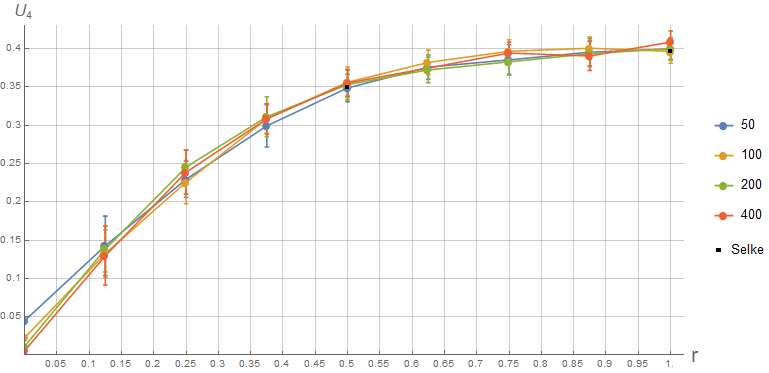
\includegraphics[width=100mm]{Sections/Images/CumulantOBC.png}
    \caption{График зависимости значения кумулянта Биндера в крит. точке от Aspect Ratio при открытых гран. условиях}
    \label{fig:CumulOBC}
\end{figure}

\begin{figure}[!h]
    \centering
    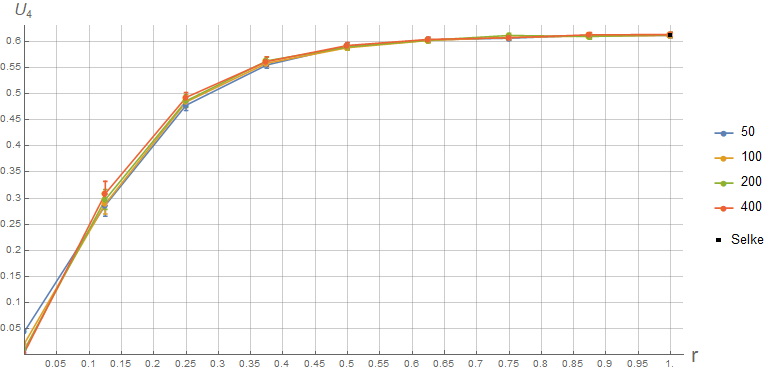
\includegraphics[width=100mm]{Sections/Images/CumulantPBC.png}
    \caption{График зависимости значения кумулянта Биндера в крит. точке от Aspect Ratio при периодических гран. условиях}
    \label{fig:CumulPBC}
\end{figure}

Крайние левые точки в отметке нуля являются расчётами для модели одномерного Изинга (где длина цепочки равна соответствующей стороне в двумерном изинге). Так, в случае открытых гран. условий (рис. \ref{fig:CumulOBC}) и периодических (рис. \ref{fig:CumulPBC}) значения кумулянта стремится к нулю с увеличением длины цепочки(см. Проект6.pdf\cite{Git}).
Черными точками отмечены значения критического кумулянта из работы Уолтера Сельке - 0.396 ± 0.002 для квадратной модели и 0.349 ± 0.002 для прямоугольной с отношением сторон r = 1/2 при открытых гран. условий. Для периодического случая квадратной модели критический кумулянт равен 0.61069\cite{Selke}.

Эти же значения отмечены в графиках \ref{fig:CumulOBCL} и \ref{fig:CumulPBCL} зависимости крит. кумулянта от обратной длины стороны как крайние левые (в нуле - так обозначен случай термодинамического предела).

\begin{figure}[!h]
    \centering
    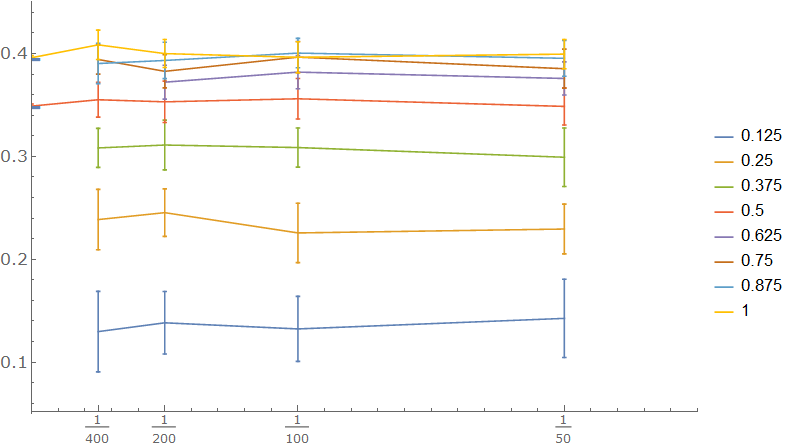
\includegraphics[width=100mm]{Sections/Images/CumulantOBCL.png}
    \caption{График зависимости значения кумулянта Биндера в крит. точке от обратной длины стороны при открытых гран. условиях}
    \label{fig:CumulOBCL}
\end{figure}

\begin{figure}[!h]
    \centering
    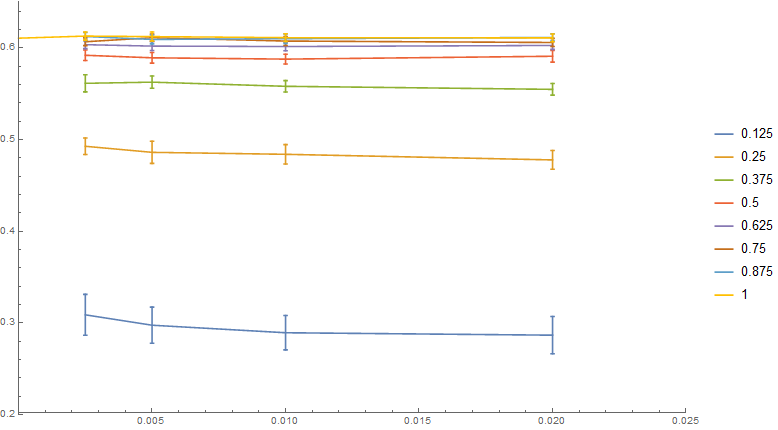
\includegraphics[width=100mm]{Sections/Images/CumulantPBCL.png}
    \caption{График зависимости значения кумулянта Биндера в крит. точке от обратной длины стороны при периодических гран. условиях}
    \label{fig:CumulPBCL}
\end{figure}

Учитывая погрешность в расчётах симуляций, зависимость от обратной длины прямоугольника 1/L не наблюдается.

\subsection{Сравнение модели Изинга и модели взаимодействующих непересекающихся блужданий}

Здесь мы рассмотрим основные понятия в модели взаимодействующих блужданий (Self-Avoiding Walks, SAWs), связанные с их формой и сравним их с прямоугольной моделью в тех же условиях. 

Важнейшим параметром в описании полученной симуляциями Монте-Карло блуждания является радиус инерции, численно равный среднему квадратическому расстоянию частиц от положения среднего арифметического центра модели (сумма $w_{k}$ в скобке)\cite{Pelissetto}:

\begin{equation}\label{eq:Rg}
    R^{2}_{g} = \frac{1}{N+1} \sum^{N}_{i=0}\left(w_{i} - \frac{1}{N+1}\sum^{N}_{k=0}w_{k}\right)^2 = \frac{1}{2(N+1)^{2}}\sum^{N}_{i,j=0}(w_{i} - w_{j})^{2}
\end{equation}

Так же для описания формы модели применяется тензор вращения относительно центра масс - матрица, $\alpha\beta-$й элемент которой расчитывается по формуле (4) из статьи\cite{Janke_G} :

\begin{equation}\label{eq:Ten_G1}
    Q_{N,\alpha\beta} = \frac{1}{N+1} \sum^{N}_{i=0}(w_{i,\alpha} - w_{c, \alpha})(w_{i,\beta} - w_{c, \beta})
\end{equation}
где $w_{c,\alpha} - \alpha$ -я координата вектора центра масс. В случае, если начало координат расположено в центре масс (следовательно, сумма векторов точек блуждания = 0), формула $\alpha\beta-$элемента тензора упрощается и численно равна второму моменту координаты (если $\alpha = \beta$), или до среднего произведения разных координат по всем точкам блуждания.


\begin{align}\label{eq:Ten_G_C}
    Q_{N,\alpha\beta} = &\frac{1}{(N+1)} \sum_{i=0}^{N} w_{i, \alpha} w_{i, \beta} \\
    \sum^{N}_{i=0}w_{i} &= 0
\end{align}

Рассмотрим формулу \eqref{eq:Ten_G1}. Так так $w{c}$ - центра масс блуждания, то:

\begin{equation}
    w_{c} = \frac{1}{N+1} \sum_{k=0}^{N} w_{k}
\end{equation}

Так же можно представить i-й вектор блуждания как:

\begin{equation}
    w_{i} = \frac{1}{N+1} \sum_{k=0}^{N} w_{i}
\end{equation}

Это позволит нам вытащить из скобок N+1 и избавиться от неизвестного $w_{c}$

\begin{align*}
    Q_{N,\alpha\beta} = \frac{1}{(N+1)^{3}} \sum^{N}_{i=0}(\sum^{N}_{k=0}(w_{i,\alpha} - w_{k, \alpha}))(\sum^{N}_{l=0}(w_{i,\beta} - w_{l, \beta})) = \\
    = \frac{1}{(N+1)^{3}} \sum^{N}_{i=0} \sum^{N}_{k,l=0}(w_{i,\alpha} - w_{k, \alpha})(w_{i,\beta} - w_{l, \beta}) = \\
    \frac{1}{(N+1)^{3}} \sum^{N}_{i=0} \sum^{N}_{k,l=0} (w_{i,\alpha} w_{i,\beta} - w_{i,\alpha} w_{l,\beta} - w_{k,\alpha} w_{i,\beta} + w_{k,\alpha} w_{l,\beta})
\end{align*}

Расскроем суммирование у учётов зависимостей индексов:

\begin{align*}
    Q_{N,\alpha\beta} = \frac{1}{(N+1)^{2}} (\sum^{N}_{i,k=0}(w_{i,\alpha} w_{i,\beta}) - \sum^{N}_{i,l=0}(w_{i,\alpha} w_{l,\beta}) - \sum^{N}_{i,k=0}(w_{k,\alpha} w_{i,\beta}) + \sum^{N}_{k,l=0}(w_{k,\alpha} w_{l,\beta})) = \\
    \frac{1}{(N+1)^{2}} \sum^{N}_{i,k=0}(w_{i,\alpha} w_{i,\beta} - w_{k,\alpha} w_{i,\beta}) = \frac{1}{2(N+1)^{2}} \sum^{N}_{i,k=0}(w_{i,\alpha} - w_{k, \alpha})(w_{i,\beta} - w_{k, \beta})
\end{align*}
т.к. кол-во произведений координат разных векторов и одинаковых меньше в два раза. Полученная формула:

\begin{equation}\label{eq:Ten_G2}
    Q_{N,\alpha\beta} \frac{1}{2(N+1)^{2}} \sum^{N}_{i,k=0}(w_{i,\alpha} - w_{k, \alpha})(w_{i,\beta} - w_{k, \beta})
\end{equation}

совпадает с формулой (4.1) из статьи о взаимодействующих блужданиях\cite{Pelissetto}, что значит что используемое ими понятие "тензора вращения" совпадает.

\subsection{Тензор инерции и тензор вращения}

Можно заметить некоторое сходство в расчётах недиагональных элементов тензора инерции J и тензора вращения из статей\cite{Pelissetto, Yanke_G}. Действительно, для системы из N материальных точек единичной массы тензор инерции в системе центра масс рассчитывается следующим образом:

\begin{equation}
    J = \left(
    \begin{array}{ccc}
        J_{xx} & J_{xy} & J_{xz}  \\
        J_{yx} & J_{yy} & J_{yz} \\
        J_{zx} & J_{zy} & J_{zz}
    \end{array} \right)
\end{equation}

\begin{align}
    J_{xy} &= J_{yx} = -\sum_{i=1}^{N} x_{i} y_{i} \\
    J_{yz} &= J_{zy} = -\sum_{i=1}^{N} y_{i} z_{i} \\
    J_{xz} &= J_{zx} = -\sum_{i=1}^{N} x_{i} z_{i} 
\end{align}

В тоже время, формулы диагональных элементов принципиально отличаются:

\begin{align}
    J_{xx} &= \sum_{i=1}^{N} y_{i}^{2} + z_{i}^{2} \\
    J_{yy} &= \sum_{i=1}^{N} x_{i}^{2} + z_{i}^{2} \\
    J_{zz} &= \sum_{i=1}^{N} x_{i}^{2} + y_{i}^{2}
\end{align}

Сравнивая с формулой элементов тензора вращения в системе центра масс \eqref{eq:Ten_G_C}, можно заметить, что недиагональные элементы тензоров отличаются знаком и усреднением в тензоре вращения. Диагональные же элементы "противоположны" друг другу:
в тензоре инерции они обозначают осевые моменты инерции (относительно $O\alpha$, и поэтому обозначенные моменты одной координатой ($J_{\alpha\alpha}$ используют сумму квадратов отличных от $\alpha$ координат.

Таким образом, элементы тензора вращения в системе центра масс в трехмерном простанстве можно представить как:

\begin{equation}
   Q_{\alpha\alpha} = \frac{1}{N}\sum^{N}_{i=1}w_{i,\alpha}^2 = \frac{1}{N} \left(\sum_{i=1}^{N}x_{i}^{2} + y_{i}^{2} + z_{i}^{2} - J_{\alpha\alpha}\right) = R^{2}_{g} - \frac{1}{N} J_{\alpha\alpha}  
\end{equation}

где $w_{i,\alpha}$ - $\alpha$-я координата радиус-вектора i-й материальной точки.

\begin{equation}
    Q_{\alpha\beta} = -\frac{1}{N} J_{\alpha\beta},\ \ \alpha \neq \beta
\end{equation}

Тогда матричный вид формулы тензора вращения через тензор инерции будет:

\begin{equation}
    Q = R_{g}^{2} * E - \frac{1}{N} J
\end{equation}
где E - это единичная матрица порядка, совпадающим с размерностью данной модели Dim.

Мы знаем, что симметричная матрица (какой являются и Q, и J) всегда диагонализируема, а базис из собственных векторов - ортогонален. Пусть S - матрица перехода в жорданов базис тензора инерции. Произведём переход в этот базис для тензора вращения:

\begin{equation*}
    S^{T}QS = S^{T} (R_{g}^{2} * E - \frac{1}{N} J) S = R^{2}_{g} * S^{T}ES-\frac{1}{N} * S^{T}JS
\end{equation*}

Матрица S - ортогональна, следовательно $S^{-1} = S^{T}$, поэтому:

\begin{equation}
    S^{T}QS = R^{2}_{g} * E - \frac{1}{N} * J_{D}
\end{equation}

где $J_{D}$ - диагонализированная матрица тензора инерции. Очевидно, что полученная в правой части матрица - диагональная. Следовательно, матрица в левой части так же получилась диагональной полсе перехода в новый базис и жорданов базис тензоров инерции и вращения одинаковы, пусть и с разными собственными значениями. Соответствующие собственные значения матриц в жордановом базисе будут равны:

\begin{align*}
    (S^{T}QS)_{ii} = Q_{D, ii} = R^{2}_{g} - \frac{1}{N}J_{ii},\ \ i=1..Dim
\end{align*}

Стоит подчеркнуть, что если жорданов базис составлен так, что собственные значения тензора инерции в матрице упорядочены по неубыванию, то в тензоре вращения собственные значения в матрице в этом базисе же будут упорядочены по невозрастанию.

\subsection{Показатели формы блуждания из тензора вращения}

Так как полученная матрица симметричная, то существует такой поворот, преобразующий её в диагональную (т.е., приводящий систему в Жорданов базис с собственными значениями по диагонали, и нулевыми недиагональными элементами), причём так, чтобы значения на диагонали были положительными и упорядоченными по невозрастанию.

В нашем двумерном случае, 

\begin{equation*}
    Q_{N} = \left(
    \begin{array}{cc}
      q_{1} & 0 \\
      0 & q_{2}
    \end{array} \right),\ 0 < q_{2} \leq q_{1}
\end{equation*}

Отметим так же, что сумма диагональных элементов тензора вращения равна квадрату радиуса вращения и инвариантна. Тогда определим ещё один показатель формы:

\begin{align*}
    s_{1} &= \frac{\la q_{1} \ra_{N}}{\la R_{g}^{2} \ra_{N}}\\
    s_{2} &= 1 - s1 = \frac{\la q_{2} \ra_{N}}{\la R_{g}^{2} \ra_{N}}\\
    r12 &= \frac{s1}{1-s1}
\end{align*}

Учитывая, что в $s_{1}$ и $s_{2}$ значения в числителе и знаменателе являются квадратами средних квадратичных значений, то следует вывод, что $\sqrt{r_{12}}$ является знакомым нам отношением сторон из предыдущего подраздела, только в данном случае это отношение не сторон прямоугольника, а полуосей эллипса инерции, который образует полученая симуляциями модель-блуждание.

\begin{figure}
\begin{minipage}[h]{0.5\linewidth}
     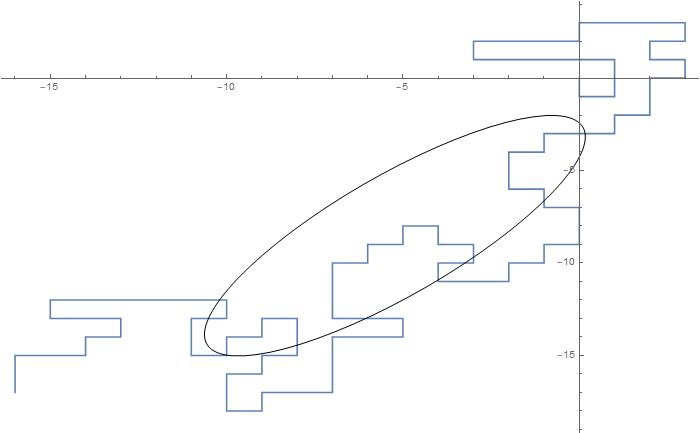
\includegraphics[width=\linewidth]{Sections/Images/GyrationEllipse.png}
\end{minipage}
\hfill
\begin{minipage}[h]{0.5\linewidth}
    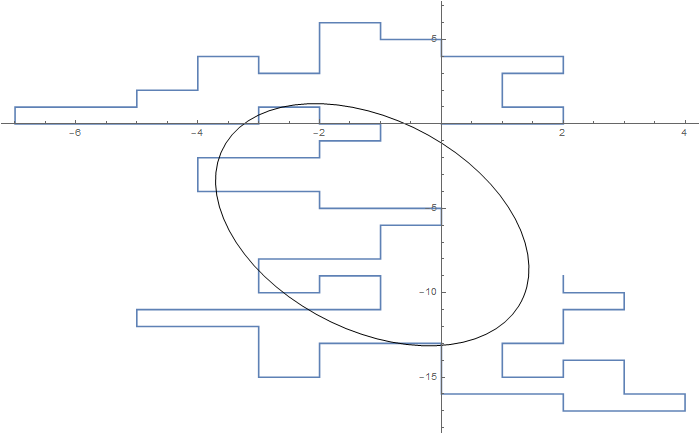
\includegraphics[width=\linewidth]{Sections/Images/GyrationEllipse2.png}
\end{minipage}
\vfill
\begin{minipage}[h]{0.5\linewidth}
     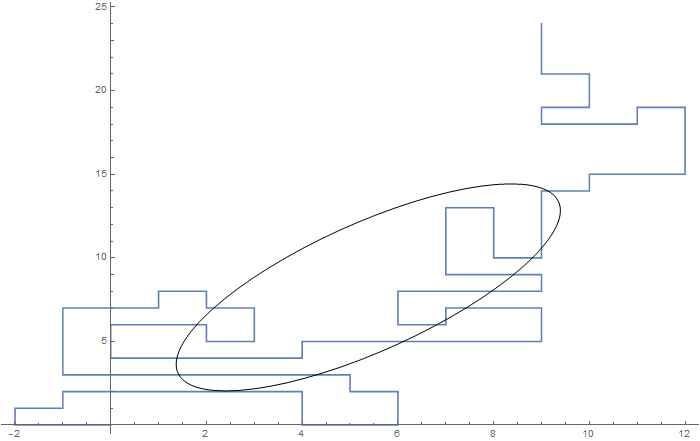
\includegraphics[width=\linewidth]{Sections/Images/GyrationEllipse3.png}
\end{minipage}
\hfill
\begin{minipage}[h]{0.5\linewidth}
    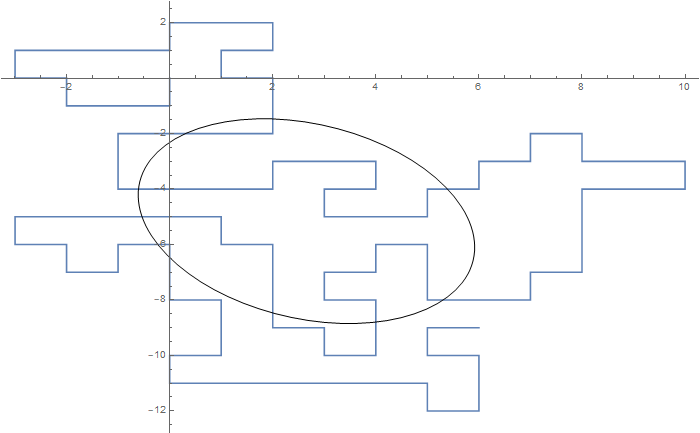
\includegraphics[width=\linewidth]{Sections/Images/GyrationEllipse4.png}
\end{minipage}
    \caption{Примеры работ симуляции по коду из Проект9.pdf\cite{Git}}
    \label{fig:my_label}
\end{figure}

